\documentclass[a4paper, 12pt]{report}

\usepackage[latin1]{inputenc}
\usepackage[T1]{fontenc}
\usepackage[sc]{mathpazo}
\usepackage[english]{babel}
\usepackage{graphicx}
\usepackage{color}
\usepackage{array}
\usepackage[margin=2.5cm]{geometry}
\usepackage{hyperref}
\usepackage{enumitem}

\usepackage{blindtext}
\usepackage[ttdefault=true]{AnonymousPro}

\usepackage[toc]{appendix}

\usepackage{standalone}

\usepackage{cleveref}
\crefname{section}{\S}{\S\S}
\Crefname{section}{\S}{\S\S}

\newcommand{\skippage}{\newpage\null\newpage}

\newcommand*{\titleTH}{ % title page
\begingroup
\raggedleft
\thispagestyle{empty}
{\Large Pavel Berkovich}\\[0.167\textheight] \centering
{\huge \texttt{N0NaMe\_}}\\[\baselineskip]
{\Large Peer-to-peer conversation security \\ using KleeQ} \\
\begin{figure}[h]
    \centering
    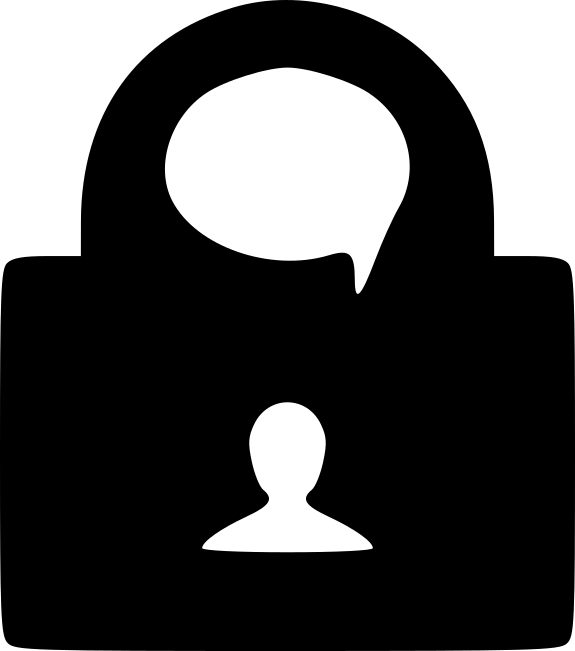
\includegraphics[width = 0.8\textwidth]{lock_chat.png} 
\end{figure}
{\large Computer Science Tripos, Part II}\\ \vspace{3mm}
{\large St John's College} \\ \vspace{3mm}
{\large 13th May, 2016}
\vfill
\clearpage
\endgroup}

\setlength{\fboxsep}{1pt}
\setlength\parindent{0pt}

\begin{document}

\titleTH

\pagenumbering{roman} % Roman page numbering

\chapter*{Proforma}
\begin{tabular}{l >{\bfseries}l}
    Name: & Pavel Berkovich \\
    Title: & NoNaMe -- Peer-to-peer conversation security using KleeQ \\
    Examination: & Computer Science Tripos, Part II, June 2016 \\
    Approx. Word Count: & {\color{red} TODO} \\
    Project Originator: & Pavel Berkovich \\
    Project Supervisor: & Dr. Richard Clayton \\
    Special Difficulties: & None
\end{tabular}

\section*{Original Aims of the Project}
The aim of this project has been to produce an implementation of KleeQ, a peer-to-peer conversation security protocol designed for devices with limited connectivity, and evaluate its performance and practicality in the broader context of Internet messaging. The intention was to preserve the security guarantees of the original design as well as understand its limitations that could potentially be used as attack vectors. It was also expected that a useable prototype of a messaging application would be produced, to evaluate the usability implications of the design as well as demonstrate the work of the implementation.

\section*{Summary of the Work Completed}

Each of the project's aims has been successfully achieved. Despite it taking more time than expected, the protocol has been implemented in full, according to the specification, retaining all of the security properties of the design. The implementation has demonstrated some impressive performance characteristics, highlighting some of the practical benefits that the use of the protocol can offer. A prototype of a messaging system, comprising a client application as well as some external components, has been implemented and tested. \\

{\color{red} 
Re-write with more specific results (with numbers etc) after do eval???}

\pagebreak
\section*{Declaration of Originality}
I Pavel Berkovich of St John's College, being a candidate for Part II of the Computer Science Tripos, hereby declare that this dissertation and the work described in it are my own work, unaided except as may be specified below, and that the dissertation does not contain material that has already been used to any substantial extent for a comparable purpose. \\[0.8cm]
\begin{tabular}{l}
    Signed \\[0.8cm]
    Date
\end{tabular}
\vfill

\tableofcontents

\skippage

\pagenumbering{arabic} % Arabic page numbering
\pagestyle{headings}

\chapter{Introduction}
\section{Background and Motivation}
Since the times of antiquity, people have employed various mechanisms to secure information against disclosure to unintended parties. Middle Eastern scholars from as early as 600 BC are credited with the creation of substitution ciphers. The ancient Greek historian Herodotus left accounts of the use of steganographic techniques, such as hiding messages beneath a layer of wax or on a messenger's body. Other notable examples of ancient information security systems include hierogliphics, the Spartan scytale and the Caesar cipher. As the schemes for protecting information were getting more elaborate, so were the methods of breaking codes and ciphers. The Arab polymath Al-Kindi, who lived in the 800s AD, is known as the inventor of frequency analysis which remained one of the key techniques in cryptanalytics until the middle of the 20th century. \\

Largely fuelled by military and commercial applications, the competition between cryptographers and codebreakers was accelerating as humanity made technological progress. Movable type printing was invented in China around 1000 AD which made it possible to print text at a large scale. The Renaissance period in Europe was marked by the impetuous development of cryptography, including the invention of the first mechanical cipher machine by Leon Batista Aberti and the discovery of the Vigen\`{e}re cipher by Blaise de Vigen\`{e}re. The 19th century and the indusrial revolution brought us the telegraph, the Morse code and the famous laws of cryptography by the Dutch mathematician Auguste Kerckhoff. \\ 

The 20th century was the time of global wars and military conflicts which provided an additional impulse to the development of information security systems. During World War I, the stream cipher and the one-time pad were developed and used for the first time. World War II involved the use of advanced electromechanical cryptographic systems by all of the sides, with the British team of cryptologists headed by John Harper famously breaking the German Enigma cipher helping the Allied powers secure the victory. During the subsequent Cold War, the adversaries were making extensive use of electronic intelligence which led to the development of some of the cyptographic primitives that we use nowadays, including Feistel network block ciphers, Diffie-Hellman key exchange protocol and RSA public key encryption. \\

With the advent of the Internet which provided means to communicate electronically on a global scale, the demand for information security systems skyrocketed as a result of the expansion of its user base from government and military officials to businesses and ordinary people. The era of global information brought many opportunities, but was also marked by the use of information technology for malicious purposes, with cybercrime costing billions to the world economy every year. The shift to mobile computing in the 2000s meant that people were now using computers for a wider range of everyday tasks which allowed them to become more productive, but also made them more vulnerable to cyberattacks and surveillance. The 2013 revelations made by Edward Snowden suggest that governments are now using their resources to collect information about ordinary civillians on a global scale, posing a direct threat to the privacy and security of our daily lives. \\

As a result of public concern in response to these new dangers, we are now witnessing an unprecedented level of effort to develop communication systems emphasising security and privacy. In particular, there has been a major push to develop secure Internet messengers which would allow people to communicate freely, without fear of being targeted by either malicious individuals or state surveillance programmes. The author of this dissertation feels great respect for these endeavors and firmly believes that having a private conversation is a fundamental right of any human being. He therefore regards this work as his own modest contribution to the noble cause of protecting humanity from the cyber-threats it is facing today.



\section{Overview of Secure Messaging}
The aforementioned series of disclosures about the widespread state surveillance programmes led to the creation of a large number of messaging systems designed with security in mind. Some of these messengers (e.g. Telegram \footnote{\url{https://telegram.org/}}) received considerable public attention and celebrated commercial success, whilst others remained largely unknown to non-experts. It is worth pointing out that, similarly to many other information security products, secure chats present an example of what is known as a ``market for lemons'' \cite{akerlof1970lemons} \cite{anderson2001information}. In this type of market, buyers have no feasible way to assess the quality of what is offered, and success of a product is determined by other factors (e.g. low price, short time-to-market), leaving producers with no economic incentive to invest in developing high-quality solutions. For secure chats, this implies that commercial success of a messaging application is by no means a measure of its actual security. \\ 

Discussing secure messaging in more detail and comparing various solutions requires a common threat model and a systematic evaluation framework. One possible approach was proposed by Unger et al~\cite{unger2015sok} in a recent survey of the existing secure messaging systems, analysing the security, usability and ease-of-adoption trade-offs of different solutions. The study identifies three key problems that any secure messenger must solve -- trust establishment, conversation security and transport privacy. \\


Below is a more detailed discussion of each of these problem areas, mentioning some of the existing solutions and their characteristics.



%\noindent The key problems are:
%\begin{description}
%    \item[Problem 1: Trust Establishment]\hfill \\
%        How do we know that our peers are who they say they are? How do we make sure that they are not being impersonated by a malicious adversary?
%    \item[\fbox{Problem 2: Conversation Security}]\hfill \\
%        Once we are sure that we are talking to the right parties, how do we protect the security and privacy of the messages' content? In other words, how do we encrypt the messages, what data do we attach to them, and what security protocols do we perform?
%    \item[Problem 3: Transport Privacy]\hfill \\
%        What is the mechanics for actually sending the message so as to hide the message metadata (e.g. sender identity, recipient identity, conversation to which the message belongs etc)?
%\end{description}
%Below is a more detailed discussion of each of these challenges, with some mentions of existing solutions and their parameters.

\subsection{Trust Establishment}
\paragraph{Definition:} \hspace{-8pt} 
\textit{Trust establishment} -- the process of making sure that communication happens with, and only with, the intended parties.

\paragraph{Explanation:}  \hspace{-8pt} 
This is the problem of making sure that our peers are who they say they are. The aim is to make it impossible for a malicious adversary to impersonate users and communicate on their behalf.

\paragraph{Common techniques and trade-offs:} \hspace{-8pt}
\begin{description}[labelindent=0.5cm, leftmargin=1.3cm]
    \item[Trust-on-First-Use (TOFU)] \hfill \\
        This method assumes the absence of adversaries at the time of initial connection and relies on memorising previously seen keys~\cite{wendlandt2008perspectives}. TOFU-based systems (e.g. TextSecure \footnote{\url{https://whispersystems.org/}}) tend to be easy to use and adopt, but do not prevent man-in-the-middle (MitM) attacks on first connection.
    \item[Manual Verification Methods] \hfill \\
        Methods in this category rely on verifying users' public keys, or some user-friendly representation thereof, out-of-band (e.g. in person). This approach is very secure, practically eliminating the possibility of a MitM attack, but has the obvious usability disadvantages. In fact, usability problems often mean that that users neglect the recommended procedures (e.g. perform key verification through unencrypted email) which results in degraded security~\cite{beautement2009compliance}.
    \item[Authority-based trust] \hfill \\
        This class of methods is widely used in the Web nowadays. The idea is to verify public keys with a trusted authority, either through public key directories or through certificates. In either case, this scheme has good usability characteristics, but leaves users unprotected from MitM attacks \textit{by the authority}. There is some ongoing work \cite{ryan2014enhanced}\cite{laurie2014certificate}\cite{melara2014coniks} aiming to fix this issue by using append-only auditable \textit{transparency logs} which would allow users to at least detect MitM attacks after the fact. This helps patch up the security to an extent, but introduces some usability issues \cite{unger2015sok}.
    \item[Web-of-Trust (WoT)] \hfill \\
        In this approach, trust is distributed rather than central. Users verify keys manualy, and then sign each other's keys and post the signatures on key servers, thereby confirming that they trust each other. Then, assuming the transitivity of the trust relation, any user can compute the set of parties they can trust (transitive closure on the trust relation). Reliance on manual verification makes WoT-based systems (e.g. PGP \footnote{\url{http://www.openpgp.org/}}) immune to MitM attacks, but hurts usability.
\end{description}

\subsection{Conversation Security}
\label{ssec:convsec}
\paragraph{Definition:} \hspace{-8pt}
\textit{Conversation security} -- the set of methods used to protect the security and privacy of the conversation's content.

\paragraph{Explanation:} \hspace{-8pt}
Once trust has been established, it is necessary to make sure that the adversary cannot see the content of the conversation, and cannot inject, modify or replay messages. Solving this problem involves deciding how to exchange keys, what format the messages should have and how they should be encrypted.

\paragraph{Common techniques and trade-offs:} \hspace{-8pt}
{\color{red}
Should I go into this much detail???}





\subsection{Transport Privacy}
\paragraph{Definition:} \hspace{-8pt}
\textit{Transport privacy} is the set of methods for hiding conversation metadata.

\paragraph{Explanation:} \hspace{-8pt}
Once we are sure that the content of the conversation is protected, we need to decide how we can hide other information about it, such as the identities of the participants, time of message transmission etc. This problem is currently considered the hardest to solve amongst the three \cite{unger2015sok}.

\paragraph{Common techniques and trade-offs:} \hspace{-8pt}
{\color{red}
Should I go into this much detail???}


\section{Substance and Aims of the Project}
The area of focus for this project is \emph{conversation security} (\cref{ssec:convsec}), which is concerned with protecting the \emph{content} of messages from the adversary. The project involves implementing and evaluating KleeQ \cite{reardon2007kleeq} -- a peer-to-peer conversation security protocol with the following security guarantees:
\begin{description}[labelindent=0.5cm, leftmargin=1.3cm]
    \item[Confidentiality] \hfill \\
        Nobody except the conversation participants can read the messages.
    \item[Intergrity of conversation] \hfill \\
        The adversary cannot inject, modify or replay messages.
    \item[Forward secrecy] \hfill \\
        A compromised key does not enable reading of previously encrypted messages.
    \item[Backward secrecy] \hfill \\
        A compromised key does not enable reading of subsequently encrypted messages.
    \item[Authorship repudiation] \hfill \\
        Given the transcript of a conversation and access to all keys, there is no computationally feasible way to prove that a given message was written by a particular participant.
    \item[Participation repudiation] \hfill \\
        Given the transcript of a conversation and access to all keys except for one user, there is no computationally feasible way to prove that this user was in a conversation with any of the others.
\end{description}

The above guarantees make KleeQ one of the most secure protocols to date. At the same time, it has some convenient usability characteristics, for example:
\begin{description}[labelindent=0.5cm, leftmargin=1.3cm]
    \item[Support for groups] \hfill \\
        Unlike many other solutions, KleeQ supports group communication natively.
    \item[Peer-to-peer (P2P)] \hfill \\
        The protocol is peer-to-peer, so no additional service provider is required.
    \item[Support for asynchrony] \hfill \\
        It is possible to send messages to disconnected peers, to be delivered when they go back online again.
    \item[Unreliable network resilience] \hfill \\
        The protocol was originally proposed for devices with transient connectivity, so it assumes that the network can delay, drop or re-order messages.
\end{description}

Whilst having an unconventional design, KleeQ strikes a good balance between security characteristics and usability, which seems to be the key trade-off in secure messaging at the moment. \\

The authors of KleeQ (Reardon et al, \cite{reardon2007kleeq}) described the core components of the protocol in sufficient detail, but only provided an unstable proof-of-concept implementation in Python. This project aims to build on their work, with the objectives summarised as follows:
\begin{description}[labelindent=0.5cm, leftmargin=1.3cm]
    \item[Implementation] \hfill \\
        Fill out the gaps in the protocol's description and construct a more robust implementation in Java, preserving the security features of the original design.
        
    \item[Evaluation of Performance] \hfill \\
        Use the newly created implementation to evaluate the performance of the protocol and its practicality for use in ubiquitous secure messaging.
        
    \item[Evaluation of Security] \hfill \\
        Understand the limitations of the protocol. See what further work would need to be done to eliminate the remaining attack vectors.
        
    \item[Messenger Prototype] \hfill \\
        Build a prototype of a messaging application based on KleeQ, with the view to assess the usability implications of the protocol.
\end{description}
The specifics of how the above objectives are addressed in this project are described in the next chapter.


\chapter{Preparation}


\chapter{Implementation}


\chapter{Evaluation}


\chapter{Conclusions}



\bibliographystyle{unsrt}
\bibliography{bibliography}
\addcontentsline{toc}{chapter}{Bibliography}

\begin{appendices}
\chapter{Project Proposal}
\section{Introduction and Description of the Work}
\label{intro}
The recent public outcry in response to mass surveillance programs carried out by governments around the world led to creation of multiple messaging systems which emphasised security of communication. Some have been more successful than others, but each of them has been found to have some flaws or deficiencies. Broadly speaking, there are four problems that each security-oriented messenger needs to solve:
\begin{description}
    \item[Problem 1: Contact Discovery] \hfill \\
        How do we find out at which IP addresses our peers currently reside? How do we know where to send our messages?
    \item[Problem 2: Trust Establishment]\hfill \\
        Once we know where our peers are, how do we know that they are who they say they are? How do we make sure that they are not being impersonated by a malicious adversary?
    \item[Problem 3: Conversation Security]\hfill \\
        Once we are sure that we are talking to the right parties, how do we protect the security and privacy of the messages' content? In other words, how do we encrypt the messages, what data do we attach to them, and what security protocols do we perform?
    \item[Problem 4: Transport Privacy]\hfill \\
        What is the mechanics for actually sending the message so as to hide the message metadata (e.g. sender identity, recipient identity, conversation to which the message belongs etc).
\end{description}

\vspace{\baselineskip}
\noindent
Multiple protocols, with different threat definitions and varying levels of security, have been developed for each of these tasks. The aim of this project is to explore and build on KleeQ, one of the protocols aimed at providing conversation security (Problem 3 in the list above). Given a group of trusted parties residing at known addresses, it gives the following security guarantees for their conversation:
\begin{itemize}
    \item confidentiality of message content
    \item message integrity
    \item forward secrecy
    \item backward secrecy
    \item message authorship repudiation
    \item conversation participation repudiation
\end{itemize}
KleeQ has been designed for devices with transient connectivity (e.g. communication via Bluetooth or wireless), but the ideas introduced by this protocol can be used in the general setting of group messaging over a network.

\vspace{\baselineskip}
\noindent
In this project, KleeQ will be completely re-implemented into a general-purpose network conversation security protocol, preserving the security properties mentioned above. The performance characteristics will be tested, and the use of the protocol will be demonstrated by constructing a simple demo messaging app.

\vspace{\baselineskip}
\noindent
Optionally, if time allows, an attempt shall be made to make use of the most recent and secure third-party solutions to solve Problems 1, 2 and 4 from the list above, thereby producing a full-blown secure messaging application.


\section{Resources Required}
All the development will be based on the resources provided by my own machine and the PWF. In addition, it is expected that a commercial cloud hosting service (DigitalOcean, Heroku or similar) will be used, for the purpose of hosting the server side of the application. The backup strategy involves periodically pushing the code to a private GitHub repository and keeping a hand-written project log. No other resources will be required.


\section{Starting Point}
As of the starting date of the project, the following relevant background:
\begin{itemize}
    \item Experience of programming in Java, at the level of University courses \emph{Programming in Java} and \emph{Further Java}.
    \item Understanding of cryptographic primitives and computer security fundamentals, as taught in Part IB \emph{Security I} course.
    \item Limited experience of writing server-side code in Python using Flask.
\end{itemize}
\vspace{\baselineskip}


\noindent
The successful completion of the core part of the project will require the following:
\begin{itemize}
    \item Learning about the fundamentals of conversation security, understanding what security properties it entails and what the common attack strategies are.
    \item Understanding the algorithms and data structures introduced by KleeQ.
    \item Learning to write security-oriented code in Java.
\end{itemize}

\noindent
To complete the optional part, the following will need to be done:
\begin{itemize}
    \item Understanding the most common attack strategies employed by adversaries against secure messengers.
    \item Reading research papers and technical documentation describing the APIs presented by the third-party libraries in use.
\end{itemize}


\section{Substance and Structure of the Project}
\subsection{Core Part}
The core part of the project will involve re-implementing KleeQ, to make it a universal conversation security protocol. Initially, it will be necessary to obtain a deep understanding of how KleeQ operates which will be done by reading the relevant research material, as well as studying the source code of the current implementation. Then, the parts of the protocol which require re-designing to allow network communication (as opposed to ad-hoc communication via Bluetooth or similar) will be identified, and the necessary design decisions will be made. The next step will be implementing the protocol in Java and testing it locally. At that point, additional checks will be made to ensure that the new implementation retains all the security properties of the original one and, if necessary, eliminate the possible loopholes in the code.

\vspace{\baselineskip}
\noindent
The next step will be turning the result of the above into a simple desktop P2P messaging application. It is important to understand that producing a full-blown secure messaging system is outside the scope of the core part of this project -- at this stage, the aim will be to write some simple and not necessarily secure "scaffolding" code to produce a prototype, for the purposes of demonstrating the work of the new protocol implementation. In particular, it is expected that a minimalistic graphical user interface and a simple server-based contact discovery component will be implemented at this point.


\subsection{Optional Extensions}
If time allows, the most recent and secure approaches may be used to convert the aforementioned demo application into a proper secure messaging system. As mentioned in Section \ref{intro}, this would require solving the problems of secure contact discovery, trust establishment and transport privacy. These problems can be solved in the following ways:
\begin{itemize}
    \item DHT with query anonymisation for contact discovery
    \item self-auditable public key logs for trust establishment (using CONIKS)
    \item Tor-based hidden service for transport privacy and metadata hiding
\end{itemize}
All of the above are available in the form of open-source libraries which can be used in the project without major modifications.

\vspace{\baselineskip}
\noindent
In addition, an effort may be made to improve the usability of the application. With this in mind, the GUI will be refined to match the usability of the most ubiquitous messenger applications (e.g. WhatsApp, Viber, Telegram etc).




\section{Success Criteria}
There shall be two measures of success for this project:
\begin{enumerate}
    \item Implementation of a working messaging system which would be possible to use.
    \item Preservation of the security properties of the original KleeQ implementation, namely:
        \begin{itemize}
            \item confidentiality of message content
            \item message integrity
            \item forward secrecy
            \item backward secrecy
            \item message authorship repudiation
            \item conversation participation repudiation
        \end{itemize}
\end{enumerate}




\section{Timetable and Milestones}
It is important to structure the project in a way which would allow to evenly distribute the workload over the available time and minimise risks of missing deadlines. In addition, as pointed out by previous Part II students, it would be beneficial to finish the dissertation write-up at least two weeks in advance of the official deadline, to allow more time for Tripos revision. With this in mind, the following schedule has been set:


\subsection*{Weeks 1-2 (Oct 25 -- Nov 6)}
Do preliminary reading and understand the algorithms and data structures used by KleeQ, referring to the existing implementation as necessary. Identify the parts of the protocol which require modification, and design the object-oriented structure of the new implementation. Decide on which standard Java classes will need to be used. Find out what common implementation mistakes result is security loopholes. Arrange the necessary infrastructure, such as a back-up repository and cloud hosting space.

\vspace{0.7\baselineskip}
\noindent
\textit{Milestone:} The necessary knowledge of the protocol acquired, design and infrastructure ready -- can begin writing code.

\subsection*{Weeks 3-7 (Nov 7 -- Dec 11)}
Implement the protocol in Java. Test locally. Watch out for most common implementation vulnerabilities. Make sure the original security guarantees are in place.

\vspace{0.7\baselineskip}
\noindent
\textit{Milestone:} The conversation security protocol implemented and tested.

\subsection*{Weeks 9-10 (Dec 12 -- Dec 25)}
Turn the protocol implementation into a library which would be usable by third parties in their applications.

\subsection*{Week 11 (Dec 26 -- Jan 1)}
A week-long holiday is planned for these dates. No work will be done during this time.

\subsection*{Weeks 12-13 (Jan 2 -- Jan 15)}
Implement the "address book" server application to allow contact discovery. Make sure the server has the most current information about user's status. Test the practicality of KleeQ's conversation concepts.

\subsection*{Week 14 (Jan 16 -- Jan 22)}
Write-up the progress report and submit it one week ahead of the deadline.

\subsection*{Weeks 15-16 (Jan 23 -- Feb 5)}
Create a minimalistic GUI. Make sure that the cases of asynchrony (device going offline or coming back online) are adequately handled.

\vspace{0.7\baselineskip}
\noindent
\textit{Milestone:} An operational messaging application is ready. Core part of the project finished, the success criteria satisfied.


\subsection*{Weeks 17-19 (Feb 6 -- Feb 26)}
Evaluate how the protocol performs over a network under high load, and try to tune it to perform better. Refine the GUI of the prototype to allow usage by non-experts.

\vspace{0.7\baselineskip}
\noindent
\textit{Milestone:} The application looks good and the performance is satisfactory.

\subsection*{Weeks 20-21 (Feb 27 -- Mar 11)}
Implement the optional extensions as time allows. Make sure that none of the previously implemented security guarantees are broken.

\subsection*{Week 22 (Mar 12 -- Mar 18)}
A week-long holiday is planned for these dates. No work will be done during this time.

\subsection*{Weeks 23-27 (Mar 19 -- Apr 22)}
Write up the dissertation. Use the project log to recollect the details of what work has been done and how. Pay special attention to the Evaluation section, describing in detail the previously made performance measurements. Arrange regular meetings with the supervisor to receive feedback and iteratively refine the work. This part of work will take a long time, since it will be interleaved with Tripos revision over the Easter Vacation.

\vspace{0.7\baselineskip}
\noindent
\textit{Milestone:} Dissertation largely written. The supervisor and the overseers are satisfied with the content.

\subsection*{Weeks 28-29 (Apr 23 -- May 13)}
No project work is scheduled for these days -- the intention is to use this time for Tripos revision. It also provides a "safety buffer" in case more time is required, for one reason or another. If necessary, final adjustments to the text of the dissertation will be made at this time.

\vspace{0.7\baselineskip}
\noindent
\textit{Milestone:} Dissertation printed, bound and submitted at least two weeks ahead of the deadline.
\end{appendices}



\end{document}
